\chapter{Tipos de processos de produção industrial}
\label{chap:tipos_de_processo_de_producao}

A classificação dos diversos tipos de empresas industriais partindo de seus processos de produção é uma tarefa importante na concepção de novas instalações industriais, pois permite identificar e reconhecer as características básicas da empresa industrial de acordo com o seu processo produtivo. As unidades produtivas podem variar desde o volume de produção (alto, médio ou baixo) até a variedade de seus produtos (alta, média ou baixa). Por isso, pode se dizer que as variáveis volume e variedade são dependentes entre si, por exemplo, operações de alto volume em geral têm baixa variedade de produtos e vice-versa. Portanto, existe uma relação inversa entre o volume e a variedade do produto \cite{slack2009administracao}.

A Figura \ref{fig:tipos_de_processo_de_producao} mostra como os cinco tipos de processos existentes estão arranjados de acordo com o espectro variedade $\times$ volume. Além disso, as características de cada um destes processos serão descritos com base no volume e variedade, descendo pela diagonal que parte do canto superior esquerdo até canto inferior direito. Em outras palavras, os processos serão descritos a seguir partindo das empresas com uma maior variedade e baixo volume até uma empresa com baixa variedade e alto volume.

\begin{figure}[H]
  \caption{Matriz Variedade $\times$ Volume: Definindo os cinco tipos de processos produtivo.} %!ALTERAR A IMAGEM POIS FALTA LEGENDA NO EIXO Y
  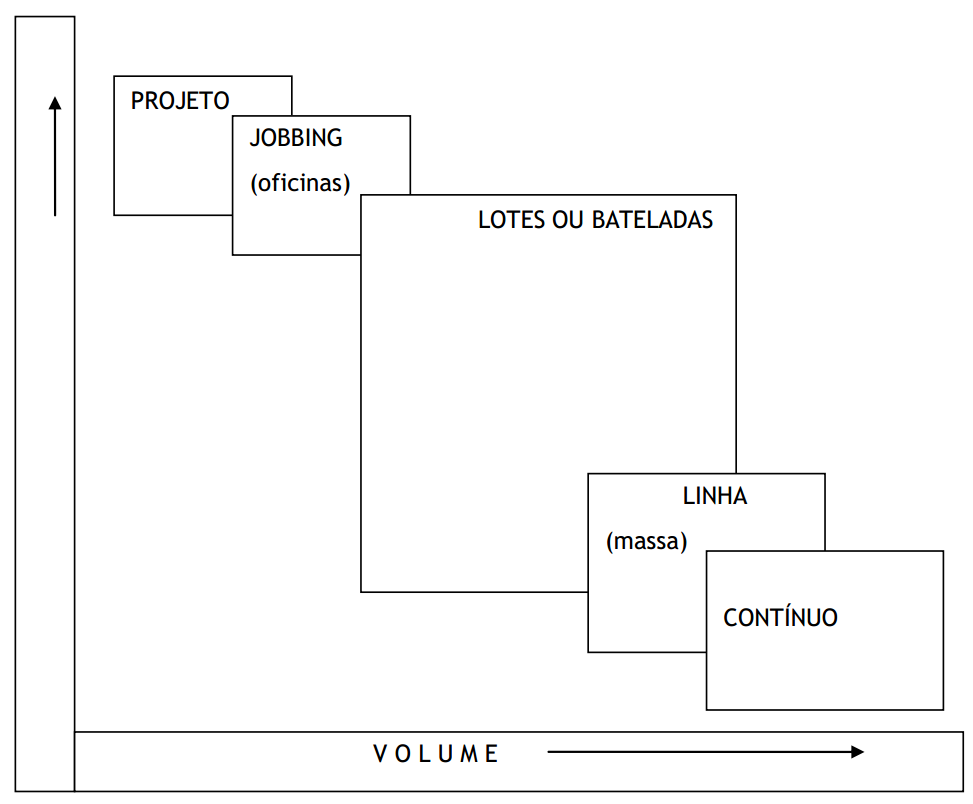
\includegraphics[width=1\textwidth]{images/tiposdeprocesso.png}
  \caption*{Fonte: Adaptado de \cite{slack2009administracao}}
  \label{fig:tipos_de_processo_de_producao}
\end{figure}

Os processos de projeto são caracterizados por possuir baixo volume, pois demoram longos períodos para serem concluídos e possuem grande variedade entre os produtos entregues. Como exemplo, cita-se a construção de uma represa. Dificilmente haverá represas parecidas devido a questões geográficas de cada represa implantada.

Os \textit{jobbings} são também conhecido como oficinas pois possuem trabalhos feitos sob encomenda e por serem semi-artesanais. Um mesmo operador pode participar do processo de construção do produto do começo ao fim. Semelhante ao projeto, esse processo também possui grande variedade e baixo volume, mas ao contrário deste o produto é, em geral, entregue ao cliente em tempo mais curto que o anterior. Um exemplo desse processo são as empresas de móveis planejados.

O processo por lotes ou bateladas, que é onde se encontra a maioria das empresas, é um estágio intermediário, das empresas que expandiram sua capacidade de produção (\textit{jobbing}) mas ainda não se encontram no estágio de grandes unidades de produção automatizada. O termo lote refere-se a produtos discretos e contáveis, como por exemplo: bolas de futebol e lápis. Por outro lado, o termo batelada trata-se de produtos contínuos, que precisam ser segregados em recipientes específicos caso haja necessidade de serem individualizados, como por exemplo: gasolina e leite.

Os processos de produção em linha/massa possuem como característica principal a linha de fabricação/montagem, onde o produto percorre as várias estações de trabalho. Nesse tipo de processo, tem-se um grande volume produzido e em contrapartida pouca variedade. Exemplo de fábrica que emprega este processo são as de fabricação de bicicletas.

Finalmente, os processos contínuos têm como característica lidarem quase sempre com fluidos (gases, pastas, líquido e misturas), que são processados no interior de tubulações e vasos fechados, além de possuírem elevada automação, o que por sua vez acaba restringindo a quantidade de mão de obra operando as máquinas. Um exemplo deste processo são as refinarias de petróleo.


\section{Aplicação Prática}
\label{sec:tipos_de_processo_de_producao_aplicacao}

A produção da SunBurn deve ser caracterizada como um processo contínuo, uma vez que a mesma produz apenas um único produto, energia elétrica, através da conversão de energia solar para energia elétrica. Tal processo ocorre de forma contínua nos diversos equipamentos utilizados, com pouco ou nenhuma intervenção humana, em grande escala. Além disso, a energia elétrica é um produto com características correlacionadas com a ideia de materiais fluidos, uma vez que ela necessita de recipientes apropriados para seu armazenamento ``individualizado'', tais como baterias e capacitores.

%! Mostrar uma imagem do processo produtivo
